\section{Preprocessing - Spliting Data}

Ο κώδικας ξεκινάει με την εισαγωγή των κατάλληλων βιβλιοθηκών συγκεκριμένα την
sklearn, pandas, matplotlib, os, numpy . Στην συνέχεια μέσω της pandas διαβάζεται
το dataset το οποίο με την εντολή describe ελέγχθηκε το μέγεθος της βάσης, ο μέσος
όρος κάθε στήλης και ο μέγιστος αριθμός σε κάθε στήλη. Με την εντολή \textbf{data.isnull().sum().head}
ελέγχθηκε εάν λείπουν τιμές από τις στήλες. Εφόσον όλα ήταν καλά, χωρίστηκε η βάση
σε δύο παραμέτρους/λίστες X, y. Η λίστα X περιέχει όλες τις λίστες πλήν της στήλης
"label". Από την άλλη η λίστα y περιέχει μόνο την στήλη "label". Μετά τον διαχωρισμό
της βάσης σε δύο λίστες , χρησιμοποιήθηκε η εντολή \textbf{resample} ωστε να ληφθεί ένα υποσύνολο του dataset , συγκεκριμένα περίπου το $24\%$ του αρχικού. Πάρθηκε αυτή η απόφαση λόγω ανεπαρκούς μνήμης του συστήματος στο οποίο "έτρεξε" ο κώδικας. 
Mετα την επιτυχή ολοκλήρωση τoυ \emph{downsampling} , ορίστηκαν
τέσσερις παράμετροι με βάση τις δύο λίστες με την εντολή X train, X test, y train, y
test = train test split(X downsampled, y downsampled, random state=40).
Στην συνέχεια χρησιμοποιήθηκε η εντολή \textbf{StandardScaler} στις λίστες Χ train, X test, η οποία τυποποιεί  τα χαρακτηριστικά αφαιρώντας τη μέση τιμή και κλιμακώνοντας τη διακύμανση, ώστε να είναι πιο έυκολο να χρησιμοποιηθούν αργότερα από τα μοντέλα. 

\section{Train SVM (linear, rbf) Models before KCPA and LDA}

Επειδή έγινε \emph{downsample} του dataset, πάρθηκε η απόφαση να αναπτυχθούν δύο μοντέλα συγκεκριμένα το \textbf{Linear SVM} και \textbf{RBF SVM}

\subsection{Linear SVM}
Αναπτύχθηκε το πρώτο μοντέλο, όπως και στην 1η εργασία το οποίο είναι το γραμμικό SVM, και
τυπώθηκε το ποσοστό ακρίβειας στο training και στο testing του μοντέλου. To train accuracy είναι 1 ενώ το test
accuracy είναι 0.91. Ο χρόνος εκπαίδευσης του μοντέλου ήταν περίπου 5.4 seconds.

\subsection{RBF SVM}
Το δεύτερο μοντέλο που υλοποιήθηκε ήταν το RBF SVM. Και εδώ τυπώθηκαν τα ποσοστά
ακρίβειας στο training και στο testing του μοντέλου. To train accuracy είναι 0.9857 ενώ το test accuracy είναι 0.962. Ο χρόνος εκπαίδευσης του μοντέλου ήταν περίπου 15.7 seconds.

\section{KPCA}

Αφού δημιουργήθηκε μία υποτηπώδης βάση για την σύγκριση των \textbf{SVM} χωρίς να έχει χρησιμοποιηθεί πάνω στα δεδομένα \textbf{KPCA}, στην συνέχεια εισάχθηκαν οι κατάλληλες εντολές μέσω της sklearn για να εφαρμοστεί η \textbf{KPCA} με δύο διαφορετικούς Κernels (RBF, Sigmoid) στις λίστες Χ train και Χ test (μετά την τυποποίηση τους).


\subsection{KPCA with RBF Kernel}

\subsubsection{Visualization of KPCA}
Αρχικά έπρεπε να βρεθεί ο αριθμός των components που θα κρατηθούν ώστε να έχουμε το $95\%$ της πληροφορίας του. Αυτό επιτεύχθηκε με την βοήθεια του διαγράμματος \ref{f:g1}, στο οποίο φαίνεται πόσα components πρέπει να βάλουμε στον αλγόριθμο του \textbf{KPCA} ώστε να κρατήσουμε την πληροφορία που ζητάμε. Έτσι μέσω αυτού του διαγράμματος και με την επαλήθευση του με την βοήθεια της εντολής \textbf{loc} της βιβλιοθήκης pandas βρέθηκε το πλήθος των χαρακτηριστηκών που πρέπει να κρατηθούν , που είναι 579.


\begin{figure}[ht]
	\centering
	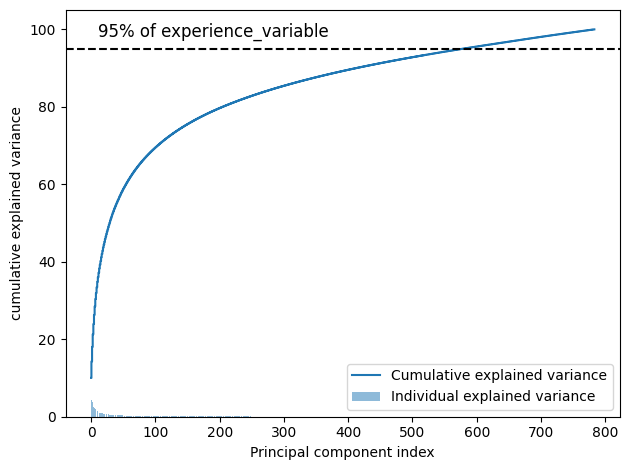
\includegraphics[width=1\linewidth]{Images data1/KPCARBFplot.png}
	\caption{ Διάγραμμα Cumulative Variance - Principal Components   }
	\label{f:g1}	
\end{figure}
\clearpage
\subsubsection{Building KPCA with the right components}

Στην συνέχεια υλοποιήθηκε ο αλγόριθμος με τον κατάλληλο αριθμό component, και παράχθηκε ένας διάγραμμα σύγκρισης μίας τυχαίας εικόνας της mnist, στην συγκεκριμένη περίπτωση φαίνεται το νούμερο \emph{6}, πριν την \textbf{KPCA} και μετά \ref{f:g2}. Παρατηρείται, ότι στην δεξιά εικόνα φαίνεται το νούμερο \emph{6} παρόλο που είναι αλλοιωμένη, οπότε η επιλογή διατήρησης του $95\%$ της πληροφορίας που υπήρχε στο αρχικό dataset (Χ train), δεν μετατρέπει την νέα λίστα (X train \textbf{KPCA}) σε άχρηστη πληροφορία για τα μοντέλα που θα εκπαιδευτούν στην συνέχεια.


\begin{figure}[ht]
	\centering
	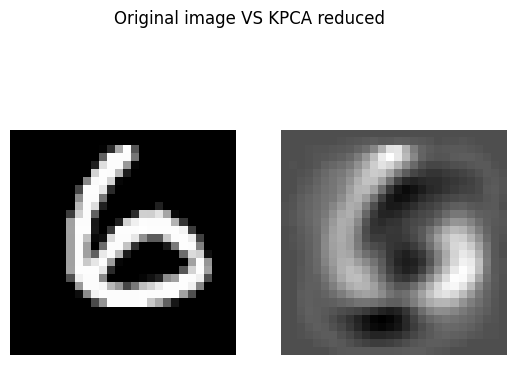
\includegraphics[width=1\linewidth]{Images data1/kpcavsoriginal.png}
	\caption{ Διάγραμμα σύγκρισης της αρχικής και μετά την KPCA εικόνας}
	\label{f:g2}	
\end{figure}

\subsubsection{Training SVM (linear, rbf) Models}

\paragraph{Linear Model}

Αναπτύχθηκε το πρώτο μοντέλο, το οποίο είναι το γραμμικό SVM, και
τυπώθηκε το ποσοστό ακρίβειας στο training και στο testing του μοντέλου. To train accuracy είναι 0.94 ενώ το test
accuracy είναι 0.92. Ο χρόνος εκπαίδευσης του μοντέλου ήταν περίπου 8.4 seconds.

\paragraph{RBF Model}

Το δεύτερο μοντέλο που υλοποιήθηκε ήταν το RBF SVM. Και εδώ τυπώθηκαν τα ποσοστά
ακρίβειας στο training και στο testing του μοντέλου. To train accuracy είναι 0.97 ενώ το test accuracy είναι 0.9362. Ο χρόνος εκπαίδευσης του μοντέλου ήταν περίπου 17.6 seconds.
\newpage

\subsection{KPCA+LDA with RBF Kernel}

Το επόμενο βήμα στην εργασία ήταν να υλοποιηθεί ο αλγόριθμος LDA πάνω στις λίστες που παράχθηκαν μέσω του \textbf{KPCA}
\subsubsection{Searching the best component  and building LDA  }

Στην αρχή όπως και στον \textbf{KPCA}, μέσω του κώδικα, επιλέχθηκε το πλήθος των component που χρειάζονται ώστε να κρατηθεί το ίδιο ποσοστό πληροφορίας με πριν ($95\%$), ώστε στην συνέχεια να εφαρμοστεί στον αλγόριθμο, το οποίο στην συγκεκριμένη περίπτωση ήταν \emph{8}.

\subsubsection{Training SVM (linear, rbf) Models}

\paragraph{Linear Model}

Αναπτύχθηκε το πρώτο μοντέλο, το οποίο είναι το γραμμικό SVM, και
τυπώθηκε το ποσοστό ακρίβειας στο training και στο testing του μοντέλου. To train accuracy είναι 0.958 ενώ το test
accuracy είναι 0.934. Ο χρόνος εκπαίδευσης του μοντέλου ήταν περίπου 0.5 seconds.

\paragraph{RBF Model}

Το δεύτερο μοντέλο που υλοποιήθηκε ήταν το RBF SVM. Και εδώ τυπώθηκαν τα ποσοστά
ακρίβειας στο training και στο testing του μοντέλου. To train accuracy είναι 0.9548 ενώ το test accuracy είναι 0.9292.Ο χρόνος εκπαίδευσης του μοντέλου ήταν περίπου 0.9 seconds.
\clearpage
\subsection{KPCA with Sigmoid Kernel}

\subsubsection{Visualization of KPCA}
Αρχικά έπρεπε να βρεθεί ο αριθμός των components που θα κρατηθούν ώστε να έχουμε το $95\%$ της πληροφορίας του. Αυτό επιτεύχθηκε με την βοήθεια του διαγράμματος \ref{f:g3}, στο οποίο φαίνεται πόσα components πρέπει να βάλουμε στον αλγόριθμο του \textbf{KPCA} ώστε να κρατήσουμε την πληροφορία που ζητάμε. Έτσι μέσω αυτού του διαγράμματος και με την επαλήθευση του με την βοήθεια της εντολής \textbf{loc} της βιβλιοθήκης pandas βρέθηκε το πλήθος των χαρακτηριστηκών που πρέπει να κρατηθούν , που είναι 579.


\begin{figure}[ht]
	\centering
	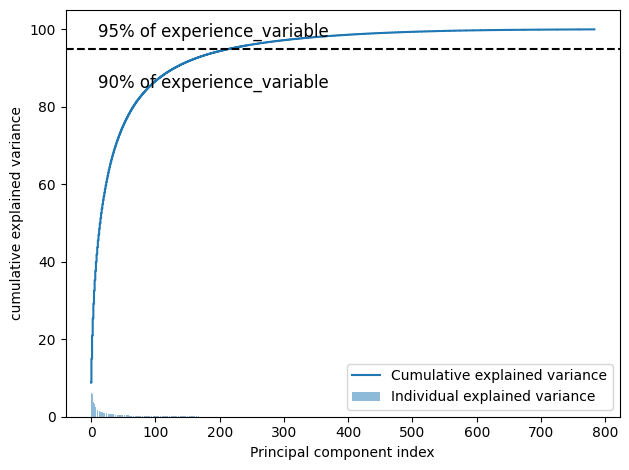
\includegraphics[width=1\linewidth]{Images data1/KPCAsigmplot.png}
	\caption{ Διάγραμμα Cumulative Variance - Principal Components  }
	\label{f:g3}	
\end{figure}

\subsubsection{Building KPCA with the right components}

Στην συνέχεια υλοποιήθηκε ο αλγόριθμος με τον κατάλληλο αριθμό component, και παράχθηκε ένας διάγραμμα σύγκρισης μίας τυχαίας εικόνας της mnist, στην συγκεκριμένη περίπτωση φαίνεται το νούμερο \emph{4}, πριν την \textbf{KPCA} και μετά \ref{f:g4}. Παρατηρείται, ότι στην δεξιά εικόνα φαίνεται το νούμερο \emph{4} παρόλο που είναι αλλοιωμένη, οπότε η επιλογή διατήρησης του $95\%$ της πληροφορίας που υπήρχε στο αρχικό dataset (Χ train), δεν μετατρέπει την νέα λίστα (X train \textbf{KPCA}) σε άχρηστη πληροφορία για τα μοντέλα που θα εκπαιδευτούν στην συνέχεια.


\begin{figure}[ht]
	\centering
	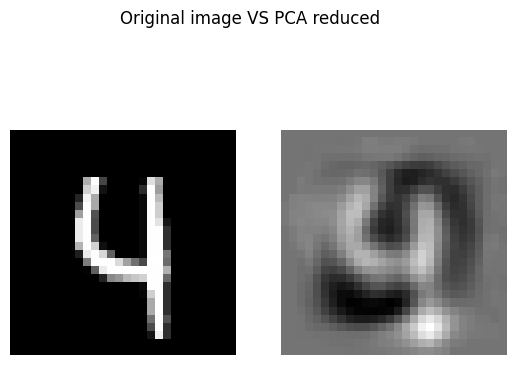
\includegraphics[width=1\linewidth]{Images data1/kpcavsoriginal1.png}
	\caption{ Διάγραμμα σύγκρισης της αρχικής και μετά την \textbf{KPCA} εικόνας}
	\label{f:g4}	
\end{figure}

\subsubsection{Training SVM (linear, rbf) Models}

\paragraph{Linear Model}

Αναπτύχθηκε το πρώτο μοντέλο, το οποίο είναι το γραμμικό SVM, και
τυπώθηκε το ποσοστό ακρίβειας στο training και στο testing του μοντέλου. To train accuracy είναι 0.926 ενώ το test
accuracy είναι 0.912. Ο χρόνος εκπαίδευσης του μοντέλου ήταν περίπου 3.1 seconds.

\paragraph{RBF Model}

Το δεύτερο μοντέλο που υλοποιήθηκε ήταν το RBF SVM. Και εδώ τυπώθηκαν τα ποσοστά
ακρίβειας στο training και στο testing του μοντέλου. To train accuracy είναι 0.999 ενώ το test accuracy είναι 0.9596. Ο χρόνος εκπαίδευσης του μοντέλου ήταν περίπου 6.3 seconds.
\newpage

\subsection{KPCA+LDA with Sigmoid Kernel}

Το επόμενο βήμα στην εργασία ήταν να υλοποιηθεί ο αλγόριθμος LDA πάνω στις λίστες που παράχθηκαν μέσω του \textbf{KPCA}
\subsubsection{Searching the best component  and building LDA  }

Στην αρχή όπως και στον \textbf{KPCA}, μέσω του κώδικα, επιλέχθηκε το πλήθος των component που χρειάζονται ώστε να κρατηθεί το ίδιο ποσοστό πληροφορίας με πριν ($95\%$), ώστε στην συνέχεια να εφαρμοστεί στον αλγόριθμο, το οποίο στην συγκεκριμένη περίπτωση ήταν \emph{8}.

\subsubsection{Training SVM (linear, rbf) Models}

\paragraph{Linear Model}

Αναπτύχθηκε το πρώτο μοντέλο, το οποίο είναι το γραμμικό SVM, και
τυπώθηκε το ποσοστό ακρίβειας στο training και στο testing του μοντέλου. To train accuracy είναι 0.8932 ενώ το test
accuracy είναι 0.8966. Ο χρόνος εκπαίδευσης του μοντέλου ήταν περίπου 0.9 seconds.

\paragraph{RBF Model}

Το δεύτερο μοντέλο που υλοποιήθηκε ήταν το RBF SVM. Και εδώ τυπώθηκαν τα ποσοστά
ακρίβειας στο training και στο testing του μοντέλου. To train accuracy είναι 0.9146 ενώ το test accuracy είναι 0.891. Ο χρόνος εκπαίδευσης του μοντέλου ήταν περίπου 1.8 seconds.

\newpage
\section{Συγκριση SVM μοντέλων πριν και μετα τους αλγορίθμους}
Θα συγκριθούν τα δυο SVM μοντέλα πριν την \textbf{KPCA} , με τα SVM μοντέλα που παράχθηκαν μετα την \textbf{KPCA}, και την KPCA + LDA. 
\subsection{Linear SVM}
Αρχικά θα συγκριθούν τα linear μοντέλα.
\subsubsection{Original vs KPCA with RBF Kernel}
Στα γραμμικά μοντέλα παρατηρείται ότι το train accuracy πέφτει μετά το \textbf{KPCA} που αυτό είναι καλό γιατί στο αρχικό είχαμε \emph{overfitting}, ενώ το test accuracy ανεβαίνει κατα 0.01 . Όμως παρόλο που μειώνονται τα features της λίστας απο 784 σε 579 ο χρόνος εκτέλεσης του μοντέλου ανεβαίνει κατα 3 second. Λόγω του ήδη μικρού dataset (μειωθηκε απο 42000 σε 10000 rows) μπορεί να θεωρηθεί αμελητέο.

\subsubsection{Original vs KPCA + LDA with RBF Kernel}
Στο γραμμικό μοντέλο μετά την εφαρμοφή των KPCA + LDA  παρατηρείται οτι το train accuracy κατεβαινει στο 0.958, ενώ ταυτόχρονα το test accuracy αυξάνεται κατα 0.02 (0.01 περισσότερο απο το \textbf{KPCA} γραμμικό SVM). Επίσης ο χρόνος εκτέλεσης του μοντέλου πέφτει σε τεράστιο βαθμό φθάνοντας το μισό second!.

\subsubsection{Original vs KPCA with Sigmoid Kernel}
To train accuracy πέφτει μετά το \textbf{KPCA} που αυτό είναι καλό γιατί στο αρχικό είχαμε \emph{overfitting}, παρόλα αυτά το test accuracy παραμένει σχεδόν ίδιο . Ο χρόνος εκτέλεσης του
γραμμικού SVM για το συγκεκριμένο Kernel μειώθηκε. Αυτό είναι πολυ καλό , αν έχουμε πολλά δεδομένα , για παράδειγμα αν είχαμε το αρχικό dataset (42000 Χ 784) , γιατί παράλληλα με την μείωση του χρόνου μας τα αποτελέσματα μένουν ίδια. Οπότε δεν θα χρειάζεται να αξιοποιηθούν πολυ πόροι για το μοντέλο.

\subsubsection{Original vs KPCA + LDA with Sigmoid Kernel}
Όταν εφαρμόζεται και ο αλγόριθμος LDA, τόσο το train όσο και το test accuracy πέφτουν κάτω απο 90\%, παρόλο που ο χρόνος μειώνεται στα 0.9 seconds.

\subsection{RBF SVM}
Στην συνέχεια θα συγκριθούν τα RBF μοντέλα.
\subsubsection{Original vs KPCA with RBF Kernel}
Στο RBF μοντέλο τα αποτελέσματα μειώνοντα για το \textbf{KPCA} με RBF Kernel. Συγκεκριμένα το test accuracy πέφτει κατα 0.03 μονάδες ενώ ο χρόνος αυξάνεται τα 2 seconds.

\subsubsection{Original vs KPCA + LDA with RBF Kernel}
Από την άλλη το RBF μοντέλο μετά το LDA  κρατάει σχεδον ίδα την διαφορά με το αρχικό(Original SVM) σε σύγκριση με το παραπάνω (\textbf{KPCA SVM}), ενώ πέφτει ο χρόνος εκτέλεσης του στα 0.9 seconds.

\subsubsection{Original vs KPCA with Sigmoid Kernel}
To train accuracy στο συγκεκριμένο μοντέλο, πέφτει ελάχιστα σε σχέση με το αρχικό , συγκεκριμένα στο 0.9596 έναντι του αρχικού που είναι στο 0.962. Ο χρόνος εκπαίδευσης πέφτει κάτω απο το μισό στα 6.3 seconds.

\subsubsection{Original vs KPCA + LDA with Sigmoid Kernel}
Αντιθέτως μετά την εφαρμογή του LDA το test accuracy πέφτει στο 0.891, παρόλο που ο χρόνος εκτέλεσης είναι πολύ μικρός, στα 1.8 seconds.

\section{Συγκριση αποτελεσμάτων 1ης εργασίας με τα αποτελέσματα των KPCA+LDA μοντέλων}
Τέλος συγκρίνονται όλα τα μοντέλα SVM με τα αντίστοιχα 
\subsection{Original vs KPCA +LDA}
Στην σύγκριση των SVM μοντέλων μετά την εφαρμογή των KPCA+LDA αλγορίθμων για Sigmoid και RBF Kernels , με τα αρχικά RBF SVM μοντέλα παρατηρείται μείωση του ποσοστού επιτυχίας των πρώτων είτε έχουν Sigmoid Kernel, είτε έχουν RBF Kernel παρόλο που ο χρόνος μειώνεται εξαιρετικά πολυ, απο λεπτά κατεβαίνει στα λίγα δευτερόλεπτα. Στην σύγκριση αρχικό γραμμικό μοντέλο παρατηρείται μία αυξηση για τον RBF Kernel αλλά όχι για τον Sigmoid. Τα αποτελέσματα του τελευταίου πέφτουν κάτων απο το 90\%.
\section{Συμπεράσματα}
Τα παραπάνω αποτελέσματα ενδεχομένως να οφείλονται στο γεγονός πως το συγκεκριμένο dataset είναι εύκολα διαχωρίσιμο χωρίς να απαιτείται η εφαρμογή \textbf{KPCA} και LDA. Συνεπώς, η απώλεια πληροφορίας που υφίσταται με την εφαρμογή KPCA+LDA είτε κοστίζει στην απόδοση , είτε παραμένει η απόδοση ίδια με του αρχικού SVM, που αυτό είναι καλό όταν θέλουμε να μειώσουμε τον χρόνο εκτέλεσης ενός προγράμματος.
